\section{Переход от лабораторной работы 3 к работе 4}

В лабораторной работе 3 сравнивались две последовательности. В первой исходные спектры источников и материала использовались для расчёта спектрального изображения, которое затем интегрировалось в XYZ и переводилось в CIE RGB. Во второй исходная сцена заранее переводилась в CIE RGB и изображение вычислялось непосредственно в этих трёх координатах. В работе 4 перед спектральным рендерингом добавляется обратная задача: по RGB сцены требуется построить спектры. Поэтому одинаковый внешний вид изображений ещё не подтверждает совпадения исходного и восстановленного спектров.

\begin{table}[htbp]\centering\small
\caption{Три вычислительные последовательности и их результат}
\begin{tabularx}{\textwidth}{@{}lX@{}}\toprule
Последовательность & Данные и операции\\\midrule
Lab3, image\_1 & Исходная спектральная сцена $\to$ спектральное изображение $\to$ XYZ $\to$ абсолютное CIE RGB $\to$ мониторное изображение\\
Lab3, image\_2 & Исходная сцена CIE RGB $\to$ прямой расчёт абсолютного CIE RGB изображения $\to$ мониторное изображение\\
Lab4, image\_A & Исходная сцена CIE RGB $\to$ восстановление спектров по трём базисным функциям $\to$ спектральное изображение $\to$ XYZ $\to$ абсолютное CIE RGB $\to$ мониторное изображение\\\bottomrule
\end{tabularx}\end{table}

Основные новые результаты работы 4 --- таблица и график исходного и восстановленного спектров, оценка ошибки их формы и сравнение image\_A с двумя последовательностями работы 3. Геометрия перспективной камеры, пересечение лучей со сферой, три контрольные точки и расчёт экстремумов сохраняются. Белый материал задаётся условием работы 4. Для контролируемого сравнения три пути должны использовать одинаковые геометрию, материал, формулу освещения, экспозицию и кодирование вывода. Фактически сохранённые изображения работы 3, полученные при других условиях, показываются отдельно и не подменяются пересчитанными изображениями.

\subsection{Обозначения исходных рисунков и реализация}

\begin{figure}[htbp]\centering
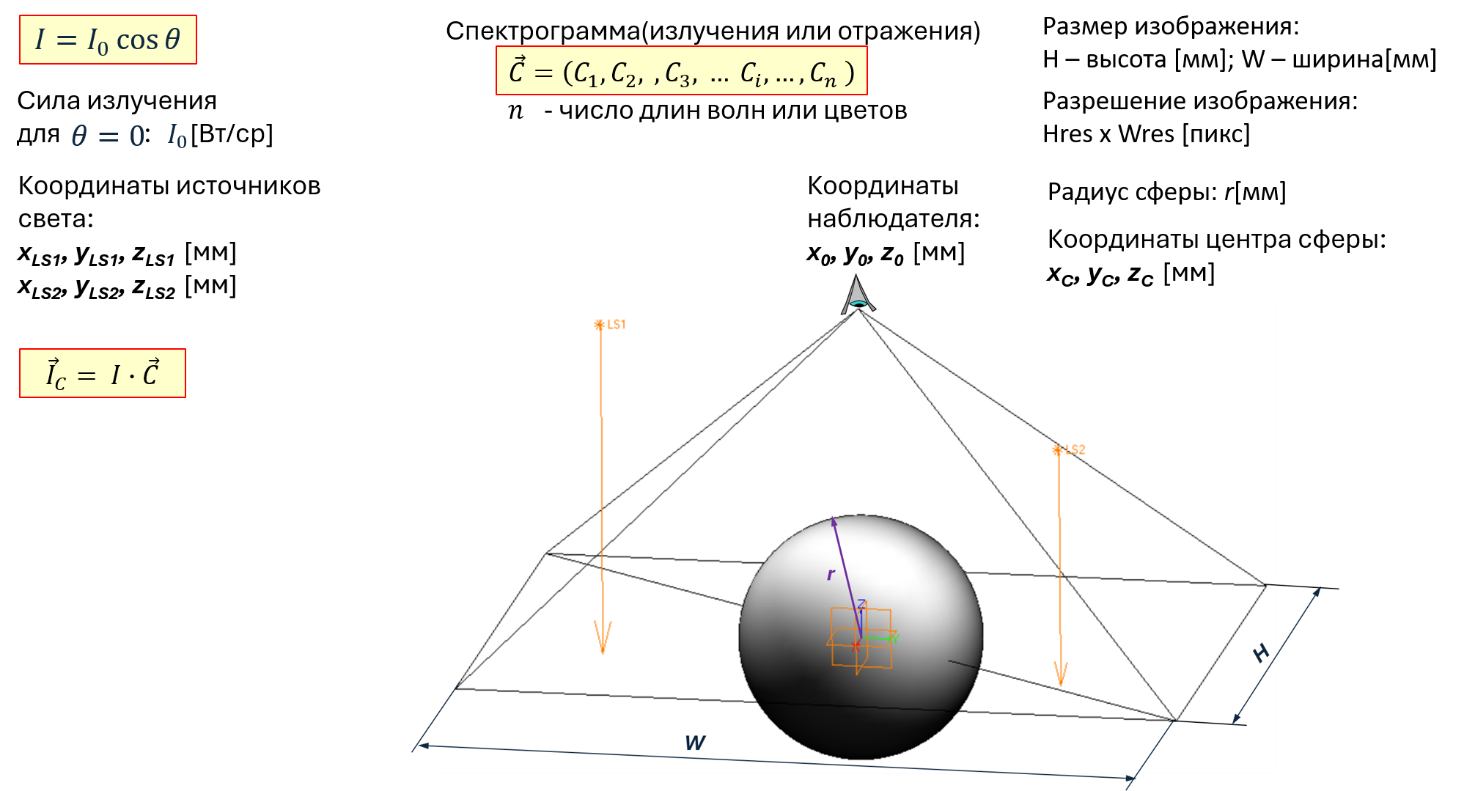
\includegraphics[width=\textwidth]{figures/assignment_1.png}
\caption{Исходный рисунок 1 из задания \code{АКГ_лр4.docx}: диаграмма источника, спектральный или цветовой вектор и геометрия сцены}
\label{fig:assignment-geometry}
\end{figure}

Вектор $\boldsymbol c=(c_1,\ldots,c_n)$ на рисунке~\ref{fig:assignment-geometry} обозначает спектрограмму излучения или отражения. Подпись объясняет $n$ как число длин волн или цветов и не задаёт конкретного пространства RGB. В данной реализации спектральный вектор имеет 41 компоненту на сетке 380--780 нм, а цветовой вектор CIE RGB --- три компоненты. Это два представления исходных данных, между которыми выполняются цветовое интегрирование и спектральная реконструкция.

\begin{table}[htbp]\centering\small
\caption{Соответствие рисунков, учебных формул и функций программы}
\begin{tabularx}{\textwidth}{@{}lX@{}}\toprule
Элемент теории & Реализация\\\midrule
$I=I_0\cos\theta$, ось источника и расстояние & \code{light_geometry} использует нормированную ось, направление от источника к поверхности и расстояние в метрах\\
Нормаль и приёмный угол $\sigma$ & \code{light_geometry} вычисляет внешнюю нормаль и направление от поверхности к источнику, обратная сторона получает нулевой вклад\\
$\boldsymbol c$ и 41 отсчёт спектра & \code{load_tables}, \code{radiance_at} и \code{calculate} хранят спектральные данные и абсолютное спектральное изображение\\
Три базисные функции и система $C\boldsymbol a=M\boldsymbol{RGB}$ & \code{reconstruct} находит коэффициенты через \code{numpy.linalg.solve} и строит восстановленный спектр\\
Интегралы XYZ и абсолютное CIE RGB & \code{spectrum_to_xyz}, \code{spectrum_to_rgb} выполняют линейные преобразования без мониторной гаммы\\
Вывод изображения & Преобразование XYZ в линейный sRGB и \code{monitor_encode} применяются после абсолютного расчёта\\\bottomrule
\end{tabularx}\end{table}

\subsection{Направления и формула освещения}

\begin{figure}[htbp]\centering
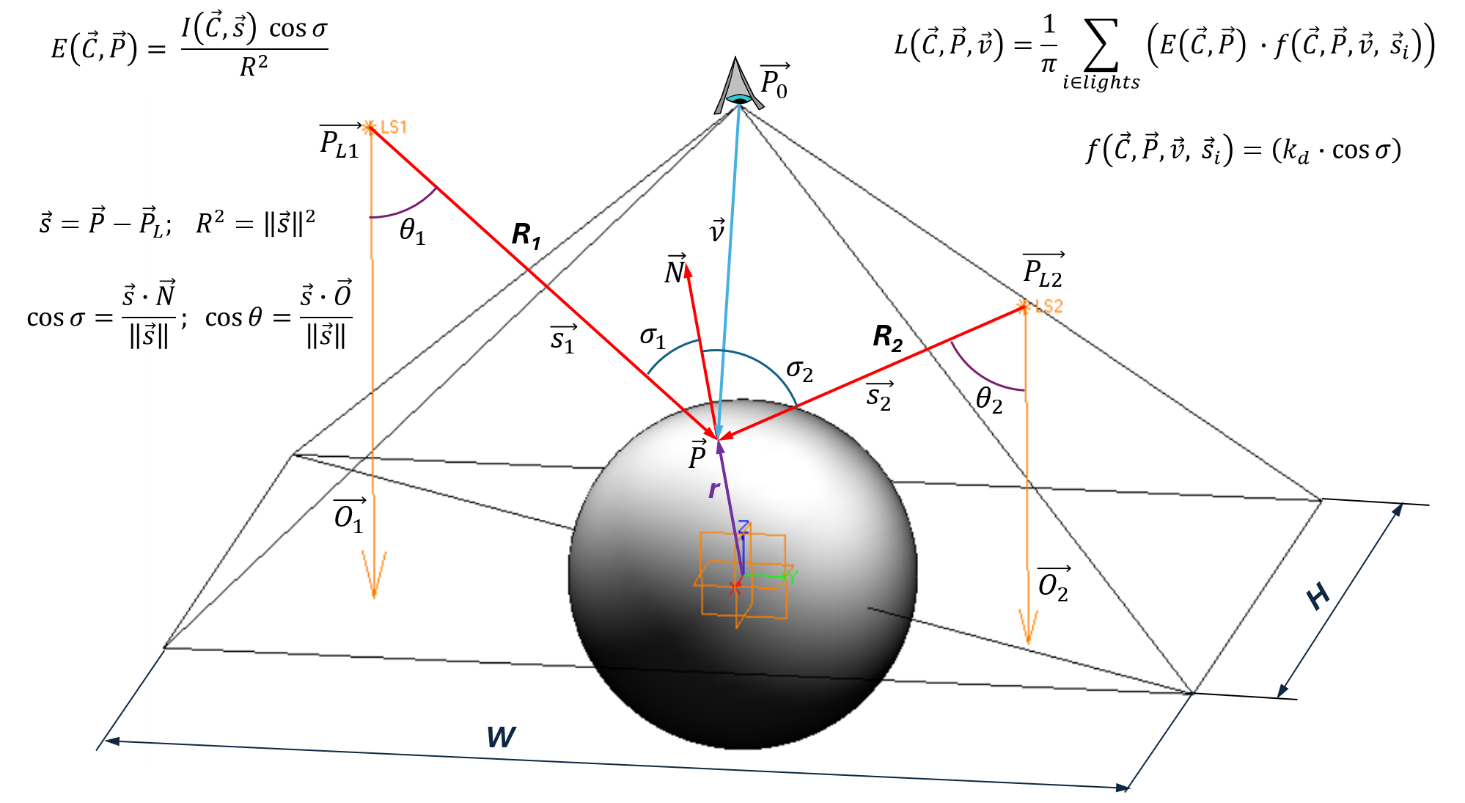
\includegraphics[width=\textwidth]{figures/assignment_2.png}
\caption{Исходный рисунок 2 из задания \code{АКГ_лр4.docx}: направления лучей, нормаль, углы и приведённые в задании формулы освещения}
\label{fig:assignment-equations}
\end{figure}

Пусть $P$ --- точка поверхности, $P_{L_i}$ --- положение источника, $\boldsymbol a_i$ --- его единичная ось, $\boldsymbol n$ --- единичная внешняя нормаль. При координатах в миллиметрах определяются
\[
 r_i=\|P-P_{L_i}\|,\qquad r_{i,\mathrm m}=r_i/1000,\qquad
 \boldsymbol e_i=\frac{P-P_{L_i}}{r_i},\qquad
 \boldsymbol l_i=\frac{P_{L_i}-P}{r_i}=-\boldsymbol e_i.
\]
С учётом диаграммы излучения источника, закона обратных квадратов и ламбертовского отражения используются
\begin{align*}
 I_{i,\lambda}&=I_{0i}\max\!\left(\boldsymbol a_i\cdot
        \frac{P-P_{L_i}}{r_i},0\right)s_{i,\lambda},\\
 E_{i,\lambda}&=\frac{I_{i,\lambda}}{r_{i,\mathrm m}^{\,2}}
        \max\!\left(\boldsymbol n\cdot\frac{P_{L_i}-P}{r_i},0\right),\\
 L_\lambda&=\frac{k_{d,\lambda}}{\pi}\sum_iE_{i,\lambda}.
\end{align*}
Здесь $s_{i,\lambda}$ --- спектральный множитель источника. Отрицательные косинусы отсекаются как отсутствие излучения или приёма с обратной стороны, а не как операция коррекции цвета.

Рисунок~\ref{fig:assignment-equations} содержит два несогласованных места. Во-первых, приёмный $\cos\sigma$ записан и в $E$, и в $f=k_d\cos\sigma$. Буквальная подстановка в приведённое там выражение $L=\sum_i(E_i f_i)/\pi$ даёт квадрат приёмного косинуса. В учебнике на печатной с.~47 формула (3.4.5.1) задаёт $L=k_dE/\pi$, поэтому в этой версии используется один приёмный косинус. Во-вторых, на рисунке задано $\boldsymbol s=P-P_L$, но нормаль направлена наружу. Для приёмного угла следует использовать противоположное направление $\boldsymbol l=(P_L-P)/r$, иначе освещённая сторона получает неверный знак. Программа явно разделяет $\boldsymbol e$ и $\boldsymbol l$. Дополнительный переключатель моделей не вводится.

\subsection{Метамерия и роль sRGB при выводе}

\begin{figure}[htbp]\centering
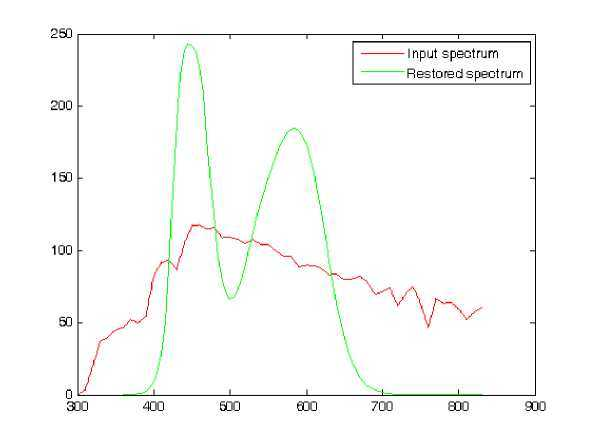
\includegraphics[width=0.82\textwidth]{figures/textbook_fig4_6.jpg}
\caption{Оригинальная иллюстрация из учебника \code{3281.pdf}, печатная с.~66, рис.~4.6: исходный D65 и его восстановление по базисным функциям. Рисунок служит пояснением метода, численные входные данные программы берутся из таблиц}
\label{fig:textbook-basis-reconstruction}
\end{figure}

Рисунок~\ref{fig:textbook-basis-reconstruction} показывает, почему сравнение работы 4 должно включать спектрограммы: различные спектры могут иметь одинаковые цветовые координаты. Восстановление по базису стандартного наблюдателя сохраняет целевые XYZ, но не обязано воспроизводить форму или интегральную энергию D65. Повторная нормировка восстановленного спектра изменила бы заданные абсолютные цветовые координаты.

Наличие матрицы \code{XYZ_TO_LINEAR_SRGB} не означает, что физическая модель вычисляется в sRGB. Спектральная реконструкция, интегралы XYZ и абсолютное CIE RGB хранятся в линейных массивах с плавающей точкой. Для них не выполняются гамма-коррекция, приведение к 0--255 и отсечение отрицательных цветовых координат. Матрица CIE RGB~$\to$~XYZ описывает расчётное пространство, а матрица XYZ~$\to$~линейный sRGB описывает основные цвета экрана. Последняя нужна только для визуализации. Нормировка, ограничение цветового охвата, мониторная гамма и округление к 8 битам применяются в конце и не изменяют сохранённые абсолютные результаты.
